\section{Quantization}
\subsection{Quantization process}
\begin{figure}[h!]
    \centering
    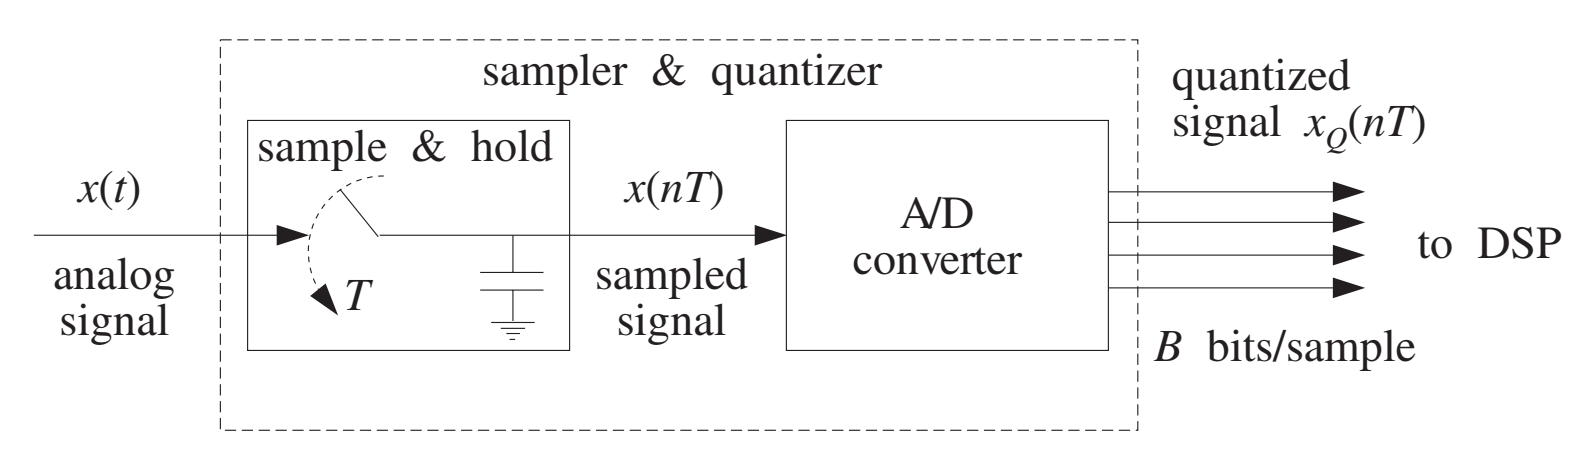
\includegraphics[width=0.5\linewidth]{img/17.png}
    \caption{Analog to digital conversion}
\end{figure}
The quantized sample $x_Q(nT)$ is represented by \textbf{B bit}, which can take $2^B$ possible values. 

An A/D is characterized by a \textbf{full-scale range R} which is divided into $2^B$ quantization levels. Typical values of R in practice are between 1-10 volts.
\begin{figure}[h!]
    \centering
    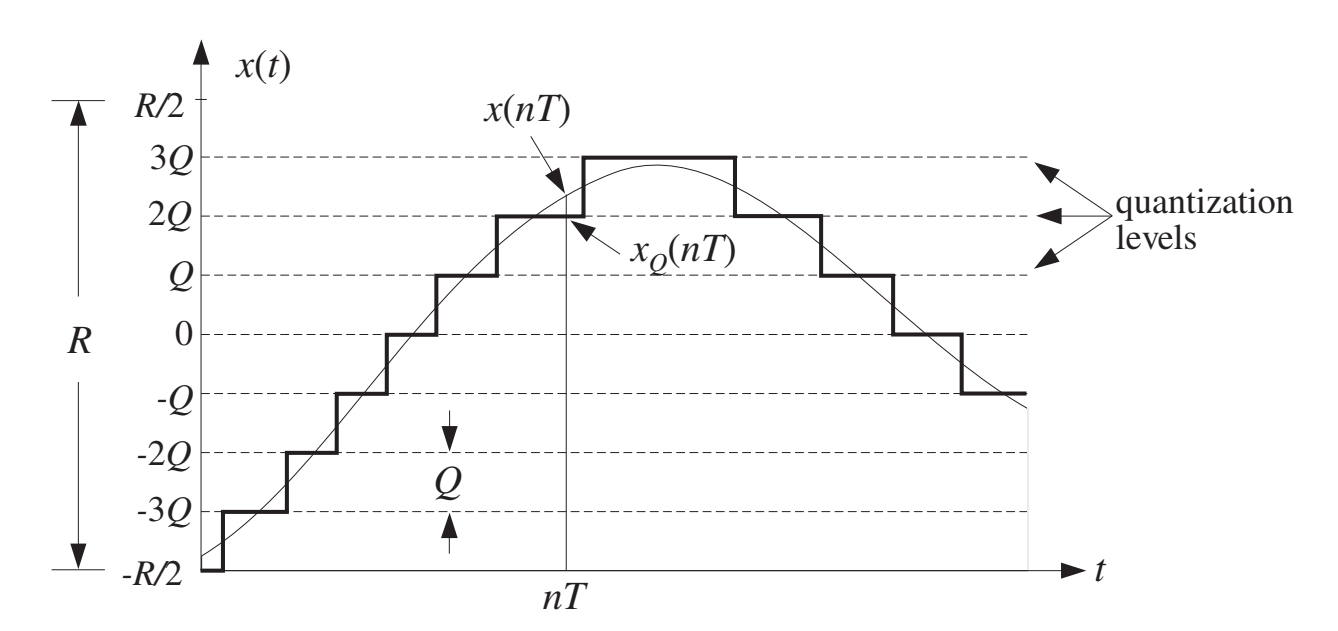
\includegraphics[width=0.5\linewidth]{img/18.png}
    \caption{Signal quantization}
\end{figure}

Quantizer resolution or quantization width (step): $Q = \dfrac{R}{2^B}$
\begin{itemize}
    \item A \textbf{bipolar} ADC: $-\dfrac{R}{2}<x_Q(nT)<\dfrac{R}{2}$
    \item A \textbf{unipolar} ADC: $0<x_Q(nT)<R$
\end{itemize}

Quantization by \textbf{\textit{rounding}}: replace each value x(nT) by the \textbf{\textit{nearest}} quantization level. 

Quantization by \textbf{\textit{truncation}}: replace each value x(nT) by its \textbf{\textit{below nearest}} quantization level.

Quantization error: $e(nT) = x_Q (nT) - x(nT)$. Consider rounding quantization: $-\dfrac{Q}{2}<e<\dfrac{Q}{2}$
\begin{figure}[h!]
    \centering
    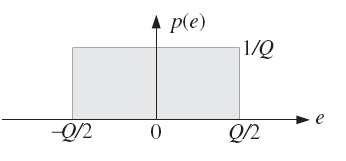
\includegraphics[width=0.3\linewidth]{img/19.png}
    \caption{Uniform probability density of quantization error}
\end{figure}

The \textbf{mean value} of quantization error: $\displaystyle \overline{e}=\int_{-Q/2}^{Q/2} ep(e)de = \int_{-Q/2}^{Q/2}e\dfrac{1}{Q}de=0$

The \textbf{mean-square error}: $\sigma^2_q = \displaystyle \overline{e^2}=\int_{-Q/2}^{Q/2} (e-\overline{e})^2p(e)de = \int_{-Q/2}^{Q/2}e^2\dfrac{1}{Q}de=\dfrac{Q^2}{12}$ (power)

Root-mean-square (rms) error: $e_{rms}=\sigma_q=\sqrt{\overline{e^2}}=\dfrac{Q}{\sqrt{12}}$

R and Q are the ranges of the signal and quantization noise, then the \textbf{signal to noise ratio (SNR)} or \textbf{dynamic range} of the quantizer is defined as
\begin{equation*}
    SNR_{dB} = 10\log_{10}\left(\frac{\sigma^2_x}{\sigma^2_q}\right)=20\log_{10}\left(\frac{R}{Q}\right)=20\log_{10}(2^B)=6B\ dB
\end{equation*}
which is referred to as \textbf{6 dB bit rule.}
\subsection{Digital to Analog Converters (DACs)}
\begin{figure}[h!]
    \centering
    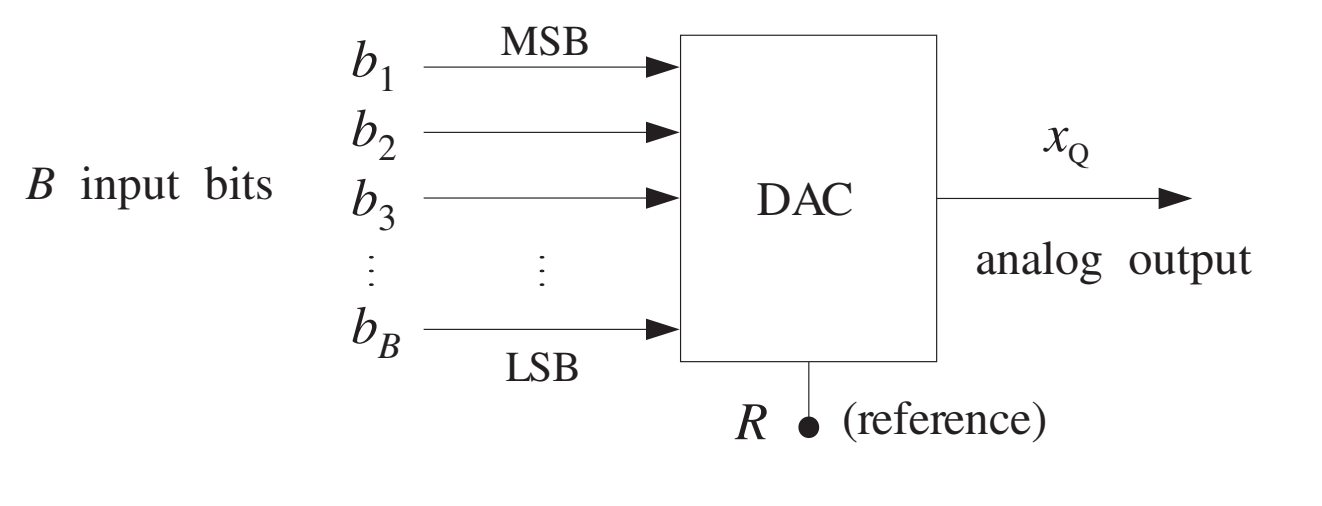
\includegraphics[width=0.5\linewidth]{img/20.png}
    \caption{B-bit D/A converter}
\end{figure}
Vector B input bits: $b=[b_1, b_2,…,b_B]$. Note that $b_B$ is the least significant bit (LSB) while $b_1$ is the most significant bit (MSB).

For unipolar signal, $x_Q \in [0, R)$; for bipolar $x_Q \in [-R/2, R/2)$.
\begin{itemize}
    \item \textbf{\textit{Unipolar natural binary}} $x_Q=R(b_12^{-1}+b_22^{-2}+...+b_B2^{-B})=Qm$ where m is the integer whose binary representation is $b=[b_1, b_2,…,b_B]$.
    \begin{equation*}
        m = b_12^{B-1}+b_22^{B-2}+...+b_B2^{0}
    \end{equation*}
    \item \textbf{\textit{Bipolar offset binary}}: obtained by shifting the $x_Q$ of unipolar natural binary converter by half-scale R/2:
    \begin{equation*}
        x_Q = R(b_12^{-1}+b_22^{-2}+...+b_B2^{-B})-\dfrac{R}{2}=Qm-\dfrac{R}{2}
    \end{equation*}
    \item \textbf{\textit{Two’s complement code}}: obtained from the offset binary code by complementing the most significant bit, i.e., replacing $b_1$ by $\overline{b_1}=1-b_1$.
    \begin{equation*}
         x_Q = R(\overline{b}_12^{-1}+b_22^{-2}+...+b_B2^{-B})-\dfrac{R}{2}
    \end{equation*}
\end{itemize}
\subsection{A/D converters}
A/D converters quantize an analog value x so that is is represented by B bits  $b=[b_1, b_2,…,b_B]$
\begin{figure}[h!]
    \centering
    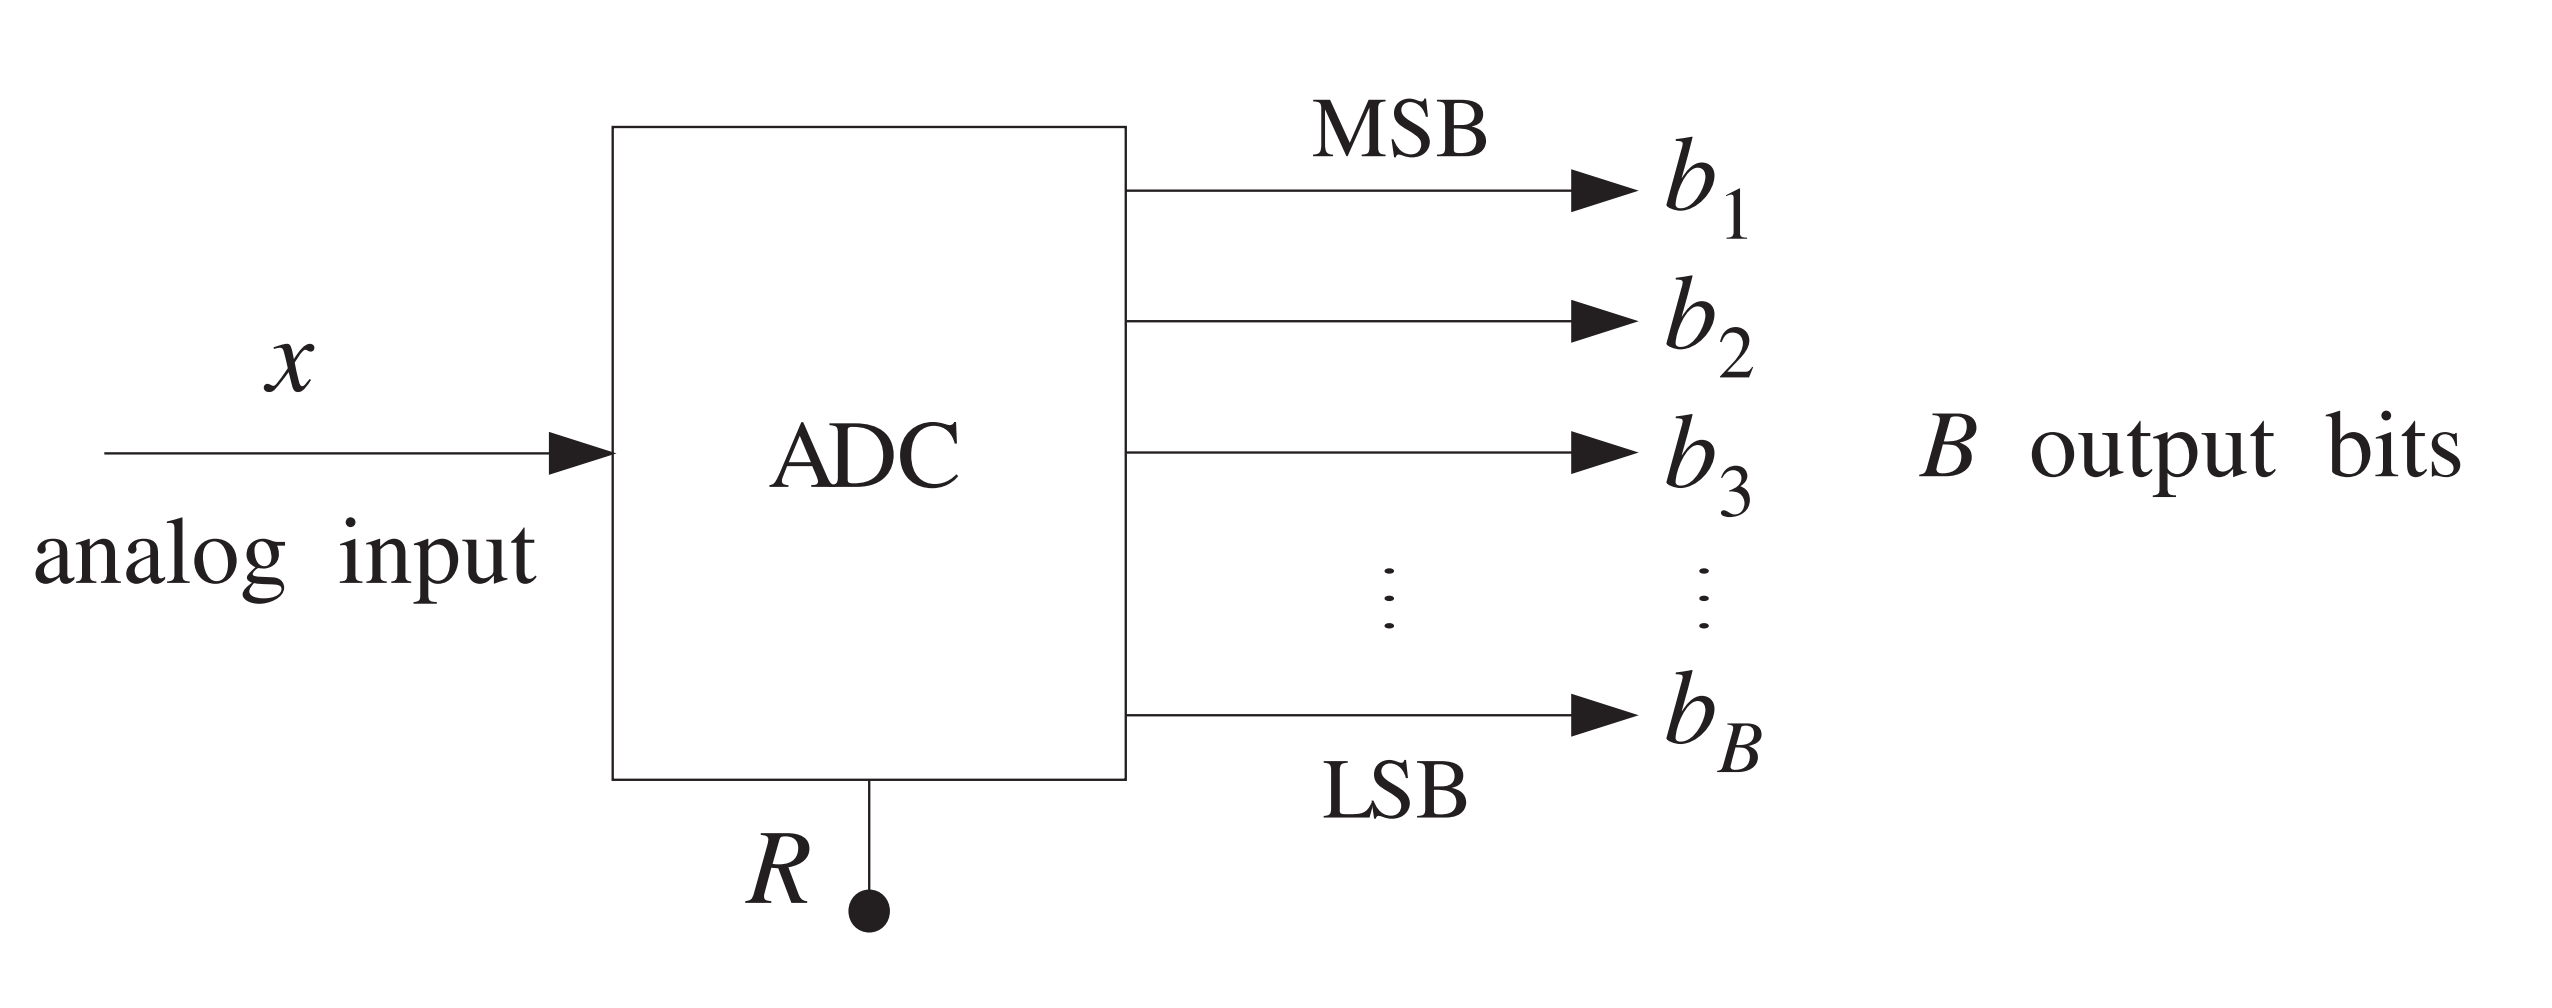
\includegraphics[width=0.5\linewidth]{img/21.png}
    \caption{B-bit A/D converter}
\end{figure}
\newpage
One of the most popular converters is the successive approximation A/D converter
\begin{figure}[h!]
    \centering
    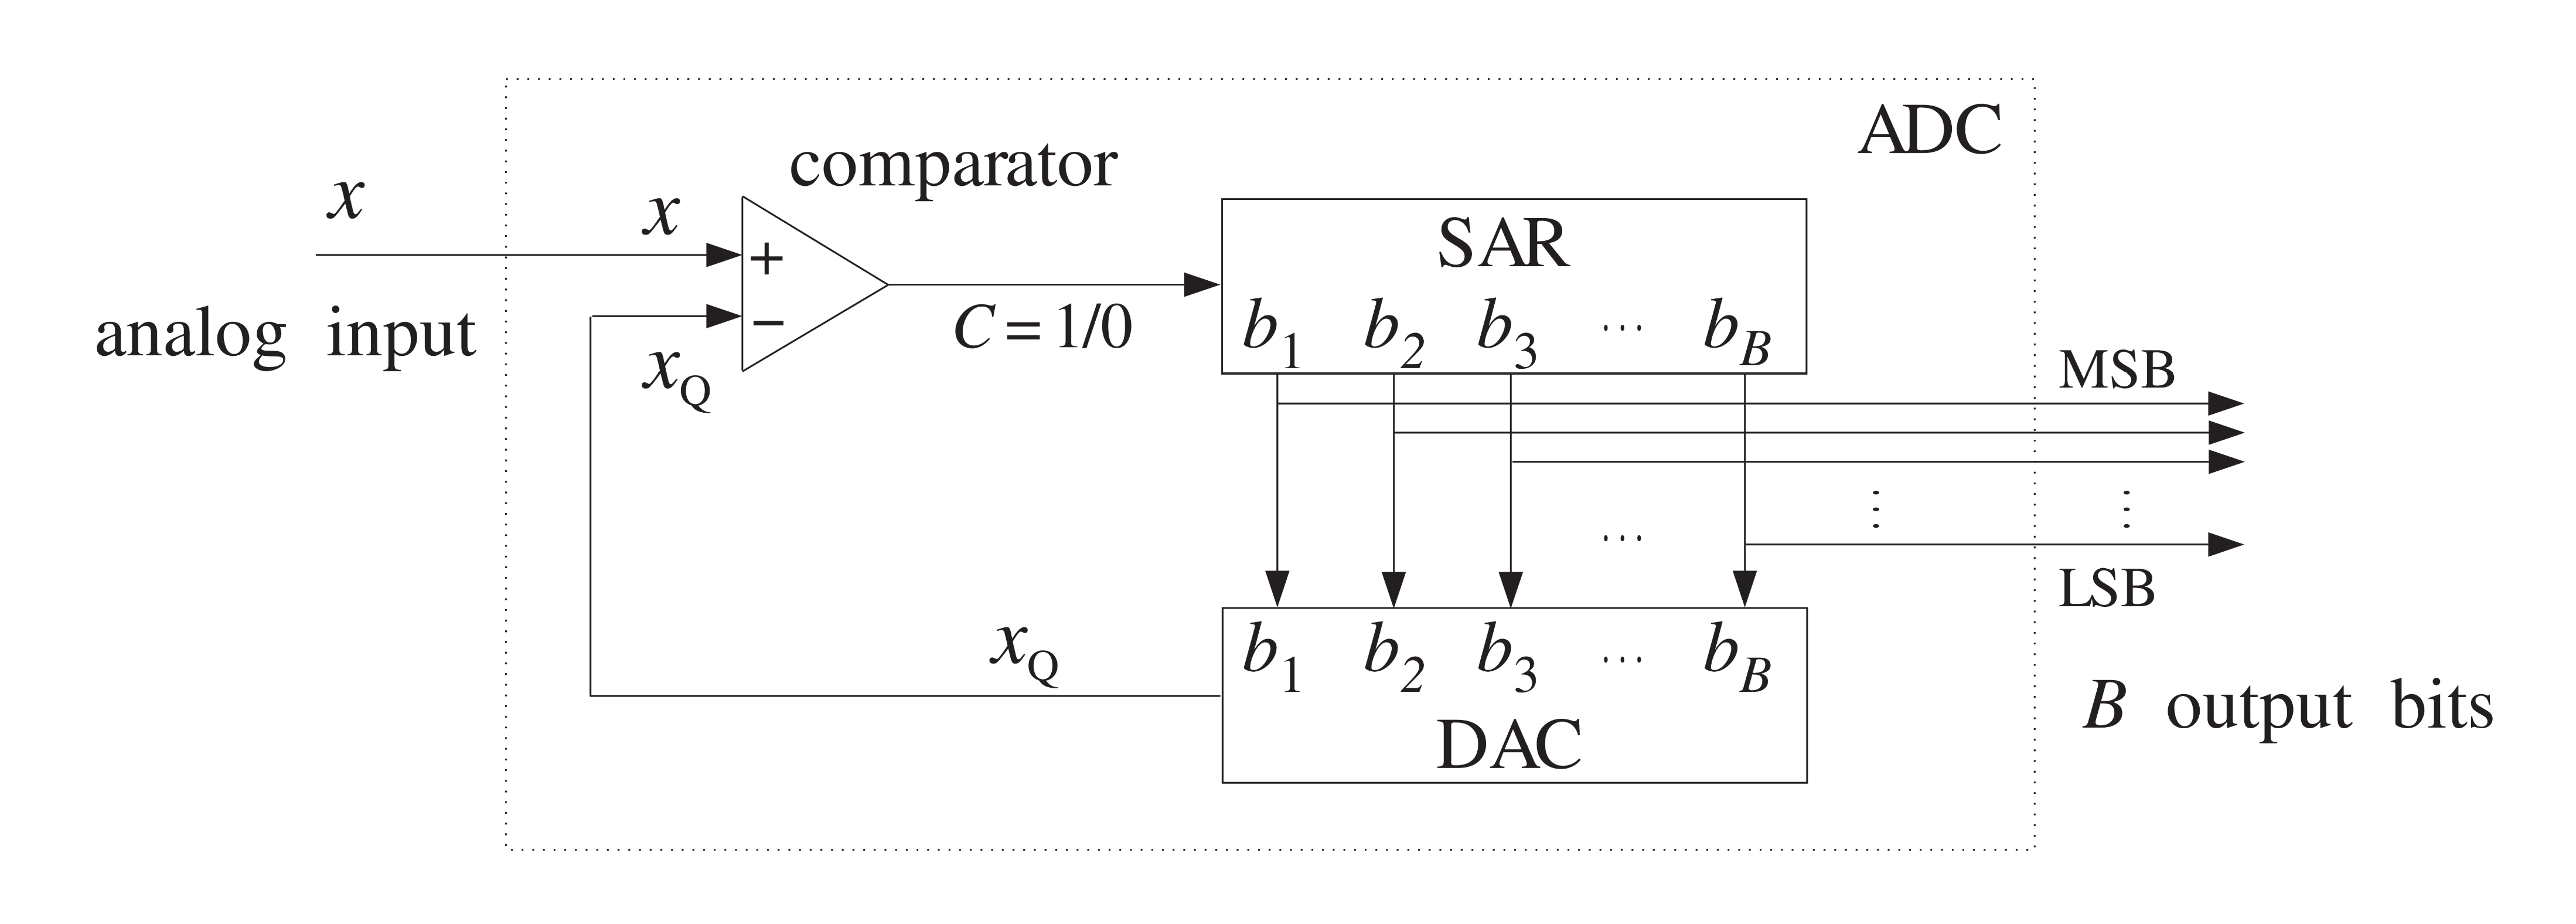
\includegraphics[width=0.5\linewidth]{img/22.png}
    \caption{Successive approximation A/D converter}
\end{figure}

After B tests, the \textbf{successive approximation register (SAR)} will hold the correct bit vector b.
\subsection{Oversampling and Noise shaping}
Because the white noise is equally distributed over the Nyquist interval with an unchanged total average power, the noise power per unit frequency interval will be reduced if the Nyquist interval is enlarged.
\begin{figure}[h!]
    \centering
    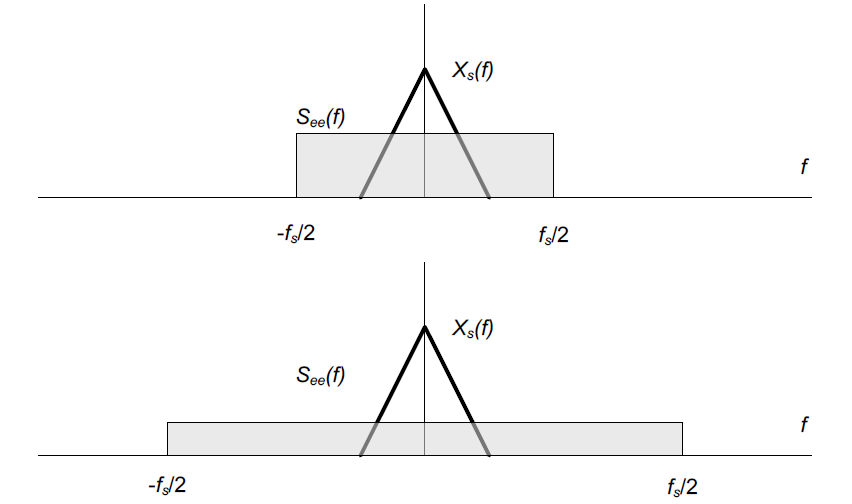
\includegraphics[width=0.5\linewidth]{img/24.png}
\end{figure}

\begin{figure}[h!]
    \centering
    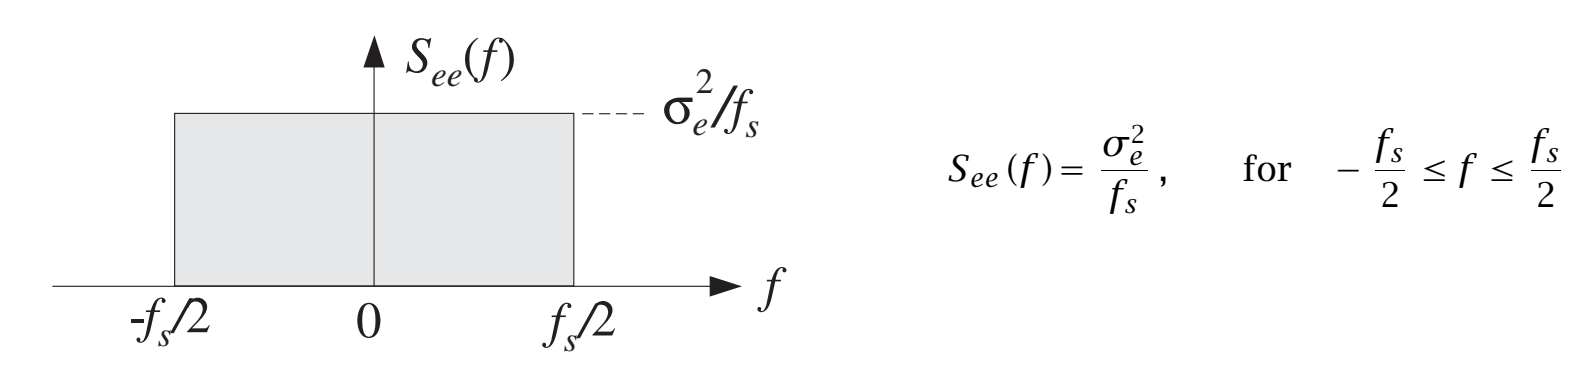
\includegraphics[width=0.5\linewidth]{img/25.png}
\end{figure}

The noise power within any Nyquist subinterval $[f_a, f_b]$ of width $\Delta f = f_b - f_a$ is given by:
\begin{equation*}
    S_{ee}(f)\ \Delta f = \sigma^2_e \dfrac{\Delta f}{f_s} = \sigma^2_e \dfrac{f_b-f_a}{f_s} 
\end{equation*}
As expected, the total power over the entire interval $\Delta f = f_s$ will be
\begin{equation*}
    \dfrac{\sigma^2_e }{f_s}f_s=\sigma^2_e 
\end{equation*}
Consider two cases, one with sampling rate $f_s$ and $B$ bits per sample, and the other with higher sampling rate $f_s’$ and $B’$ bits per sample.
\begin{figure}[h!]
    \centering
    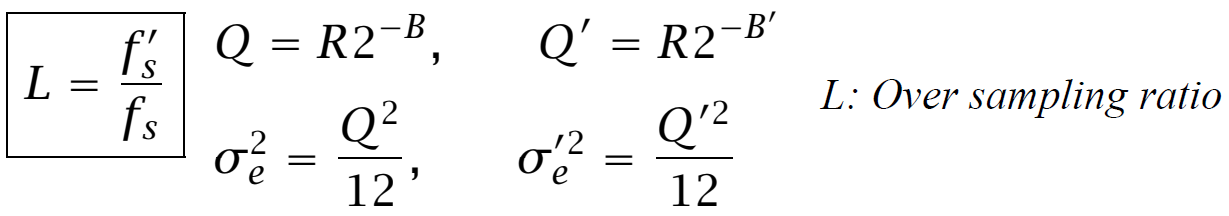
\includegraphics[width=0.5\linewidth]{img/26.png}
\end{figure}

\textbf{To maintain the same quality in the two cases, we require that the power spectral densities remain the same:}
\begin{figure}[h!]
    \centering
    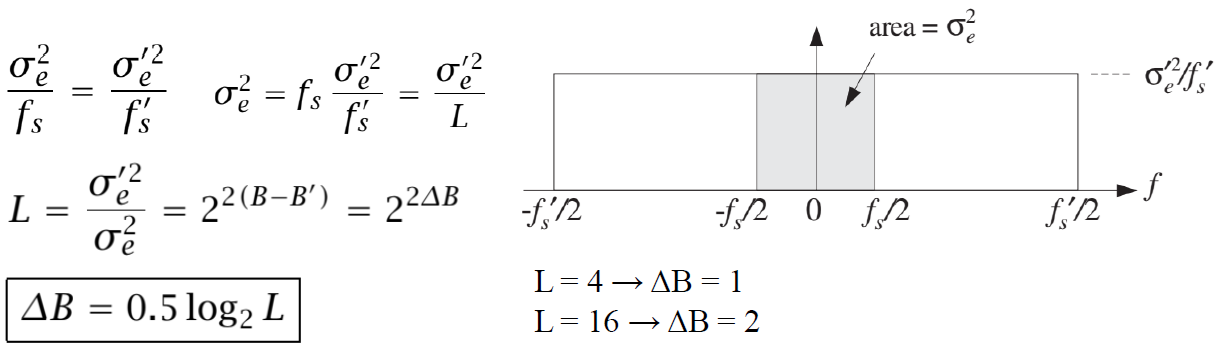
\includegraphics[width=0.5\linewidth]{img/27.png}
\end{figure}

\textbf{\textit{Noise shaping}} quantizers reshape the spectrum of the quantization noise into a more convenient shape


